\section{}


\subsection{Geometry}

The FTOF geometry is implemented through the COATJAVA geometry service.
The service provides the geant4 definitions that are read by the GEMC perl api to build the geometry database.

All scintillators are geant4 volumes.
Each scintillator is a G4Box embedded in a G4Trapezoid mother volume made of air, see \F{ftofGeometry}.

\begin{figure}
	\centering
	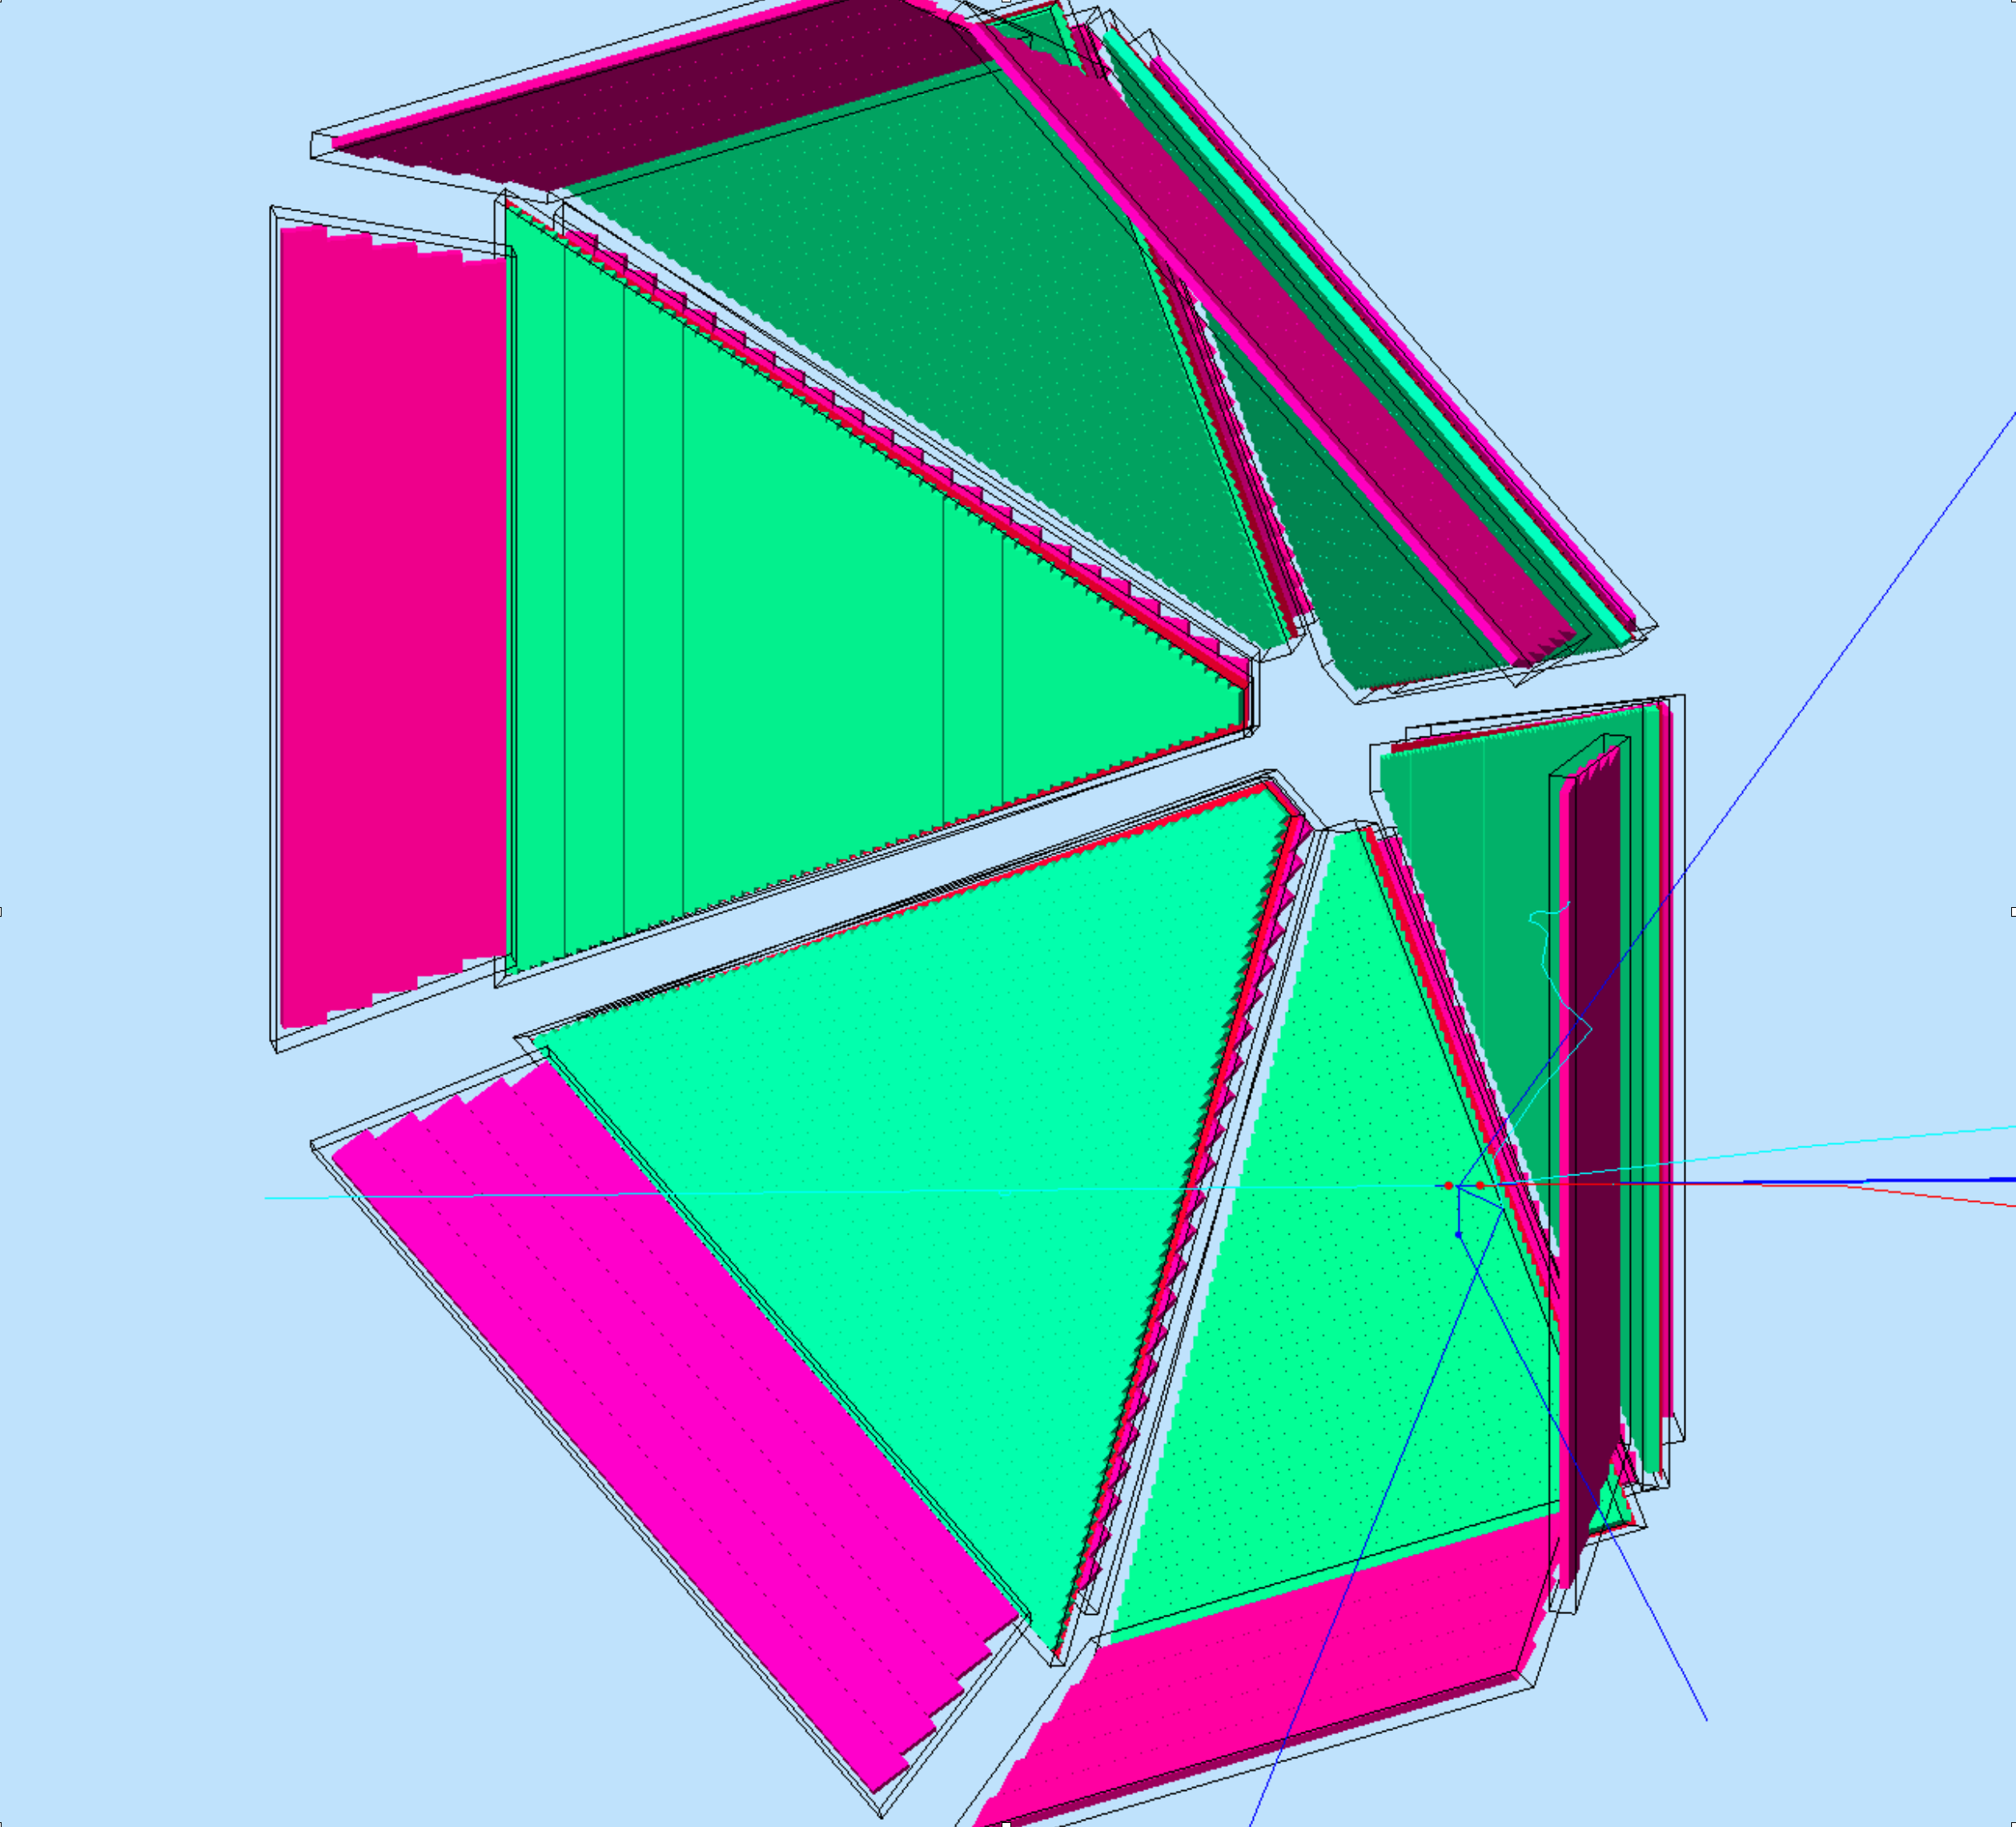
\includegraphics[width=0.95\columnwidth,keepaspectratio]{img/ftofGeometry.png}
\caption{Cherenkov light yield as a function of pion momentum and photon wavelength. The study took into account: the mirror reflectivity; the number of reflections on the mirror and Winston Cones;
the gas refraction index and the gas reflectivity as a function of wavelength; the PMT quantum efficiency; different improvements to optics and PMTs response increase. }
	\label{fig:ftofGeometry}
\end{figure}


\subsubsection{Geometry Git Location}
The github location of the gemc perl api script is 

\subsection{Calibration Constants}

\subsubsection{Summary of CCDB Table used}

\subsection{Digitization}

\subsection{Process ID}

\subsubsection{Time Window}

\subsubsection{Process Routine Git Repository Location}


